\section{Fuchsia}

\begin{figure}[H]
    \centering
    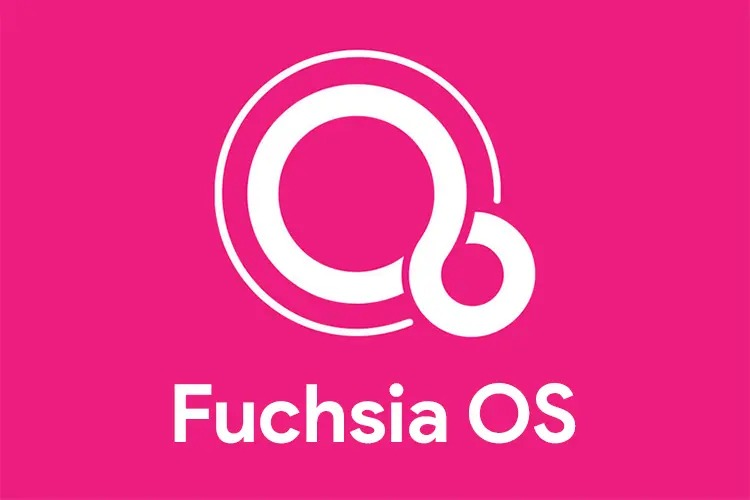
\includegraphics[width=0.35\textwidth]{figures/fuchsia.jpeg}
    \caption[Ícono de FuchsiaOS]%
            {Ícono de FuchsiaOS \citep{fuchsia2025}}
    \label{fig:fuchsia}
\end{figure}

Fuchsia OS es un sistema operativo desarrollado por Google desde 2016, diseñado como una plataforma de propósito general para dispositivos embebidos, móviles, IoT y potencialmente de escritorio. A diferencia de Android, no se basa en Linux, sino en un núcleo propio denominado Zircon \citep{zirconkernel}.  

Su arquitectura está basada en un microkernel, en el que Zircon gestiona procesos, hilos, memoria y comunicación mediante objetos e IPC, mientras que servicios como sistemas de archivos y controladores se ejecutan en espacio de usuario, favoreciendo la seguridad y modularidad \citep{fuchsiadocs}.  

Fuchsia está escrito principalmente en C++, Rust y Dart. Zircon se implementa en C/C++, mientras que la capa de interfaz gráfica se desarrolla con Flutter (Dart), lo que facilita la portabilidad a múltiples plataformas \citep{googlefuchsia}.  

Entre sus componentes clave se encuentran la gestión de procesos basada en objetos, memoria virtual con aislamiento estricto, soporte para múltiples sistemas de archivos (como MemFS, BlobFS y FAT) y un entorno gráfico con Flutter para experiencias multiplataforma \citep{zirconkernel}.  

El proyecto es mantenido principalmente por Google, con participación de la comunidad de código abierto. Su documentación oficial está disponible en Fuchsia.dev, que incluye guías técnicas, API y manuales de contribución, aunque parte del desarrollo se mantiene cerrado \citep{fuchsiacommunity}.
